\documentclass[12pt]{article}

\usepackage[utf8]{inputenc}  
\usepackage[portuguese]{babel}   
\usepackage{enumerate}
\usepackage{listings}             % Include the listings-package
\usepackage{color}
\usepackage{graphicx}
\usepackage{amsmath}


\title{Lista 01 de Processamento de Imagens}
\date{2º Período de 2021}
\author{Turma do 3º ano}



\begin{document}


\maketitle


\vspace{3em}

\begin{enumerate}



\item Considere a seguinte representação de uma imagem com 10 possíveis tons de cinza (entre 0 e 9).

\begin{figure}[h]
    \centering
    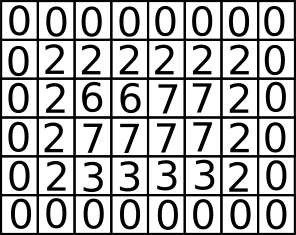
\includegraphics[width=0.40\textwidth]{img-matrix}
    \caption{Matriz de uma Imagem}
    \label{fig:img-matrix}
\end{figure}

\begin{enumerate}

\item Faça o histograma da imagem


\item Passe um filtro de média $3\times 3$ na imagem \ref{fig:img-matrix}. 
Este filtro consiste em operações locais em cada ponto da imagem, 
o pixel resultante será a média do valor dos vizinhos (incluindo ele mesmo).
Escreva a imagem resultante. 
O filtro não precisa ser aplicado nas bordas da imagem.


\end{enumerate}


\item Considere a seguinte matriz associada a uma imagem.


\[
\begin{bmatrix}
  0 &  0 &  2 &  6 &  2 &  0 \\
  0 &  0 &  2 &  6 &  2 &  0 \\
  0 &  0 &  2 &  6 &  2 &  0 \\
  0 &  0 &  2 &  6 &  2 &  0 \\
  0 &  0 &  2 &  6 &  2 &  0 \\
  0 &  0 &  2 &  6 &  2 &  0 
\end{bmatrix}
\]



\begin{enumerate}

\item Passe o filtro blur nesta matriz.

\[
\begin{bmatrix}
  1 &  1 &  1 \\
  1 &  1 &  1 \\
  1 &  1 &  1 
\end{bmatrix}
\cdot\frac{1}{9}
\]

\item Passe o filtro de sobel na matriz para detectação de bordas.

Some o resultado de passar a máscara

\[
\begin{bmatrix}
  1 &  0 &  -1 \\
  2 &  0 &  -2 \\
  1 &  0 &  -1 
\end{bmatrix}
\cdot\frac{1}{9}
\]

E o resultado de passar a máscara

\[
\begin{bmatrix}
  1 &   2 &   1 \\
  0 &   0 &   0 \\
 -1 &  -2 &  -1 
\end{bmatrix}
\cdot\frac{1}{9}
\]


\item Passe o filtro de contraste

Faça a operação entre imagens

\[\mbox{imagem original} + (\mbox{imagem original} - \mbox{imagem blur})\]

onde ``imagem original'' é a imagem original e ``imagem blur'' é o resultado de passar o filtro \textit{blur} pela imagem original




\item Faça a binarização da imagem: utilizando apenas as duas cores extremas (0 e 9), cada pixel deve receber apenas uma dessas cores. 
Na imagem resultante deve existir apenas essas cores.


\end{enumerate}






\end{enumerate}

\end{document}









